\documentclass[11pt]{article}
\usepackage[latin1]{inputenc}
\usepackage{amsmath}
\usepackage{amsfonts}
\usepackage{amssymb}
\usepackage{graphicx}
\usepackage{setspace}
\usepackage[left=1.00in, right=1.00in, top=1.00in, bottom=1.00in]{geometry}
\usepackage[english]{babel}
%\setlength{\parindent}{0pt}
\newcommand{\forceindent}{\leavevmode{\parindent=1.5em\indent}} % em = roughly width of uppercase ``M", or just over a third of a cm

\usepackage{fancyhdr}

\pagestyle{fancy}
\fancyhf{}
\rhead{University of Houston $|$ Political Science}
\lhead{Learning \LaTeX: Week 3} %% BE SURE TO CHANGE THIS EACH WEEK
\rfoot{Page \thepage}

\graphicspath{/Users/bpwaggo/Dropbox/LaTeX Workshop Series/Week 3}
%\usepackage{pdflscape} % USE THIS INSTEAD: (just after \begin{table}) \resizebox{\linewidth}{!}{

\usepackage[round]{natbib}
\bibliographystyle{apsr}

\begin{document}
	
	\title{Learning \LaTeX \\
		\vspace{1cm}
	\large Week 3: Equations, Lists, \& Numbering \\ %% BE SURE TO CHANGE EACH WEEK
		\vspace{1cm}}
	\author{Philip D. Waggoner\footnote{{\texttt{philip.waggoner@gmail.com}}. This document was prepared by Philip Waggoner for the \textit{Weekly Workshops on Learning \LaTeX}, hosted by the Deparment of Political Science, University of Houston.}}
	\date{ } % getting rid of the automatic date
	\maketitle

\newpage

\tableofcontents

\newpage

\section{Introductory Remarks}
	
\forceindent In the social sciences, we often write and use equations in our work. Whether calling a functional form of a model, generating proofs, or creating new measures of our own, we will need to be familiar with the ability to both write and include equations in the body of our text. This implies the need to understand at least basic Greek letters, as well as their appropriate usage in writing papers. As I will not teach all Greek letters and specific equations (I leave that to your statistics professors), I assume you have some level of knowledge of these letters and their proper use in statistics and scientific writing. \\

An important note: when reading equations, we read them as part of a sentence. Therefore, we need to include normal punctuation as we include equations in our work (e.g., after an equation is included, we would place a comma after it, to segue into a block of text describing each term in the equation).  Further, we will walk through how to align numerous equations, as well as where equations are placed (e.g., set apart or ``displayed" versus inserting a text within the main text). \\

Pivoting a bit, we will then discuss how to create ``bulleted" lists as well as numbered lists. These come in handy in a variety of contexts, while may require different placement and formatting within the document. As such, we will walk through proper formatting of lists in written work (e.g., centering or left-justified). \\

\textbf{Our goals for today (made using the ``itemize" environment):}

\begin{itemize}
	\item Write, insert, and reference equations in text
	\item Generate, manipulate, and format \textit{ordered} lists
	\item Generate, manipulate, and format \textit{numbered} lists
\end{itemize}

\newpage 

\section{Equations}

\subsection{Basics of Equations}

\forceindent To begin, we have two main options or modes to work with when including equations in our documents. We can either keep them in line with the text, or we can set them apart (i.e., ``display"). To include equations within the text, we need specific delimiters (e.g., ( ), \$ \$, and so on). So for example, type:\footnote{Downs, Anthony. 1957. ``An Economic Theory of Political Action in a Democracy." \textit{Journal of Political Economy}, 65(2): 135--150.} \\


\begin{figure}[!h]
	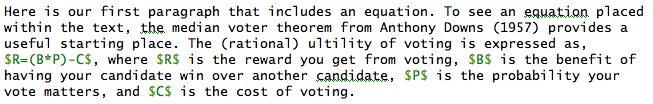
\includegraphics[scale=.5]{CODE1} \\
	\centering
\end{figure}

This code gives us a well-formatting, simple equation placed directly in the text,

\begin{figure}[!h]
	
\includegraphics[scale=.5]{OUT1} \\
	\centering
\end{figure}

So we can see that the equation is include in the same font and size right within our text as we told it to do. Notice that the italicizing of each term is done automatically by placing each term within the ``\$" delimiter. This especially comes in handy when you have more complicated terms as we will see below. \\

Now, let's see the same thing, but with a different delimter. Let's use parentheses: \\

\begin{figure}[!h]
	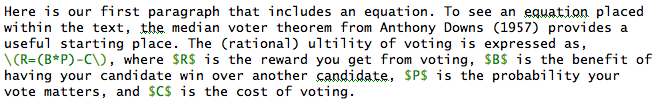
\includegraphics[scale=.5]{CODE2} \\
	\centering
\end{figure}

This code gives us, \\

\begin{figure}[!h]
	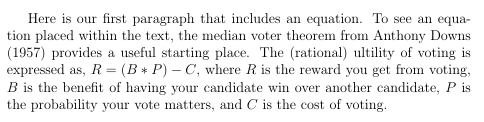
\includegraphics[scale=.5]{OUT2} \\
	\centering
\end{figure}

\newpage

As we would expect, the output is identical.\footnote{Note, that you can display equations also using a double ``\$" or also the ``math" environment, typed directly into the text. Try these out to see whether (if) things change.} \\

Now if we wanted to display the equation by setting it apart from the text, we would need a different ``mode", which is simply using brackets instead of the parentheses used above. So, to update our previous example, type: \\

\begin{figure}[!h]
	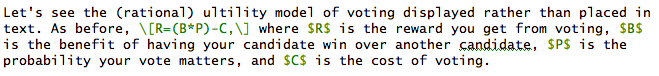
\includegraphics[scale=.5]{CODE3} \\
	\centering
\end{figure}

Now, this code gives us, \\

\begin{figure}[!h]
	
\includegraphics[scale=.5]{OUT3} \\
	\centering
\end{figure}

See that the equation is now separated from the text and displayed more prominently as we told \LaTeX\ to do by calling the brackets as our delimiters instead of parentheses. Also, note that to read the equation with proper syntax like a normal sentence, we need to place the comma within the bracket delimiter in order to keep the comma associated with the equation (displayed), rather than separated from it. \\

\subsection{Greek Letters \& Commonly Used Equations}

\forceindent With the basic intuition behind equations, let's first take a look at a few commonly used Greek letters, and see how these work while building out equations. \\

First, as with many things in \LaTeX, Greek letters are quite intuitive. Simply type the name of the letter following the command backslash. For a few examples, type a few commonly used Greek letters:

\begin{figure}[!h]
	
\includegraphics[scale=.5]{CODE4} \\
	\centering
\end{figure}

\newpage

As we would expect, this code gives us, \\

\[\alpha, \beta, \gamma, \sigma, \delta, \epsilon\]

Feel free to experiment (or look up) as many different letters as you wish. You can find many resources online. \\

Let's look at a few commonly used expressions and equations. A few are fractions, large operators (summation, products), exponents, and subscript. To write a fraction, we simply use the command ``frac". The numerator goes in the first set of braces and the denominator in the second set. To use large operators, depending on our needs, we write the command for whatever the operator does. So for summation (captial Sigma), the command is ``sum," and for products we call command ``prod" (or captial ``Pi"). For exponents, we use the carrot, the same symbol as in \texttt{R}. And naturally for subscript, we use the underscore, ``\_".\footnote{Indeed, there are many symbols used in math. These are just a few major examples. For more on this, see: \texttt{http://web.ift.uib.no/Teori/KURS/WRK/TeX/symALL.html}.} \\

To see each of these in commonly used formulas in statistics, type:

\begin{figure}[!h]
	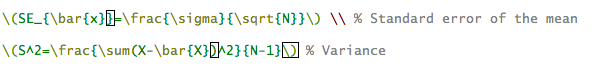
\includegraphics[scale=.5]{EQS} \\
	\centering
\end{figure}

Now we get the well-formatted equations, \\

\begin{center}

\(SE_{\bar{x}}=\frac{\sigma}{\sqrt{N}}\) \\ % Standard error of the mean

\vspace{.5cm}

\(S^2=\frac{\sum(X-\bar{X})^2}{N-1}\) \\ % Variance

\end{center}

\subsection{Numbering Equations}

\forceindent To number equations, rather than placing an equation directly in the text (either inine or displayed), we would need to use the ``equation" environment. In \LaTeX, the equation environment automatically numbers (and keeps up with) equations, as long as they are all written in the equation environment. \\

Also, like last week with tables and figures, we can give equations labels, allowing us to keep track and organized throughout, as well as reference specific equations in the main text, without worrying how many we have. We do this with the ``ref" commend. To see this and everything else we have done in practice, we will use an example from my research on measuring partisan issue prioritization: \\

\begin{figure}[!h]
	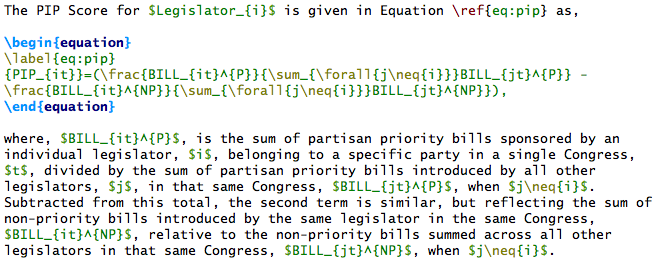
\includegraphics[scale=.5]{CODE6} \\
	\centering
\end{figure}

\newpage

And now our output with everything altogether is, \\

	The PIP Score for $Legislator_{i}$ is given in Equation \ref{eq:pip} as,

\begin{equation}
\label{eq:pip}
{PIP_{it}}=(\frac{BILL_{it}^{P}}{\sum_{\forall{j\neq{i}}}BILL_{jt}^{P}} - \frac{BILL_{it}^{NP}}{\sum_{\forall{j\neq{i}}}BILL_{jt}^{NP}}), \\
\end{equation}

where, $BILL_{it}^{P}$, is the sum of partisan priority bills sponsored by an individual legislator, $i$, belonging to a specific party in a single Congress, $t$, divided by the sum of partisan priority bills introduced by all other legislators, $j$, in that same Congress, $BILL_{jt}^{P}$, when $j\neq{i}$. Subtracted from this total, the second term is similar, but reflecting the sum of non-priority bills introduced by the same legislator in the same Congress, $BILL_{it}^{NP}$, relative to the non-priority bills summed across all other legislators in that same Congress, $BILL_{jt}^{NP}$, when $j\neq{i}$. \\

\subsection{Aligning Multiple Equations}

\forceindent Finally, if we have multiple equations that are especially complicated, or at least that we want aligned at a specific point within the equation, we need to access another nested environment. As you may expect, it is called ``align." Importantly, it works similar to the ``tabular" environment in making a table, where ``\&" symbols are used to align text. So the alignment occurs where the ampersand is placed. Also, and importantly, the align environment simultaneously numbers equations, as well as centers them in the page, similar to the ``equation" environment. And you can control the numbering with ``*" as you would with sections, subsections, and so on (see Week 1 for more on this). \\

To see this in practice, consider the following code:

\begin{figure}[!h]
	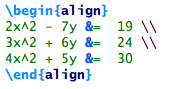
\includegraphics[scale=.6]{CODE7} \\
	\centering
\end{figure}

\newpage

This gives us the output, \\

\begin{figure}[!h]
	
\includegraphics[scale=.6]{OUT7} \\
	\centering
\end{figure}

\newpage 

\section{Lists}

\subsection{Basics of ``Itemize"}

\forceindent In \LaTeX, creating bulleted lists is a very straightforward tool to fill big needs we often have in research and writing. To create lists, we simply leverage the ``itemize" environment, where each item on the list is categorized with the ``item" command. To see this in practice, type the following:

\begin{figure}[!h]
	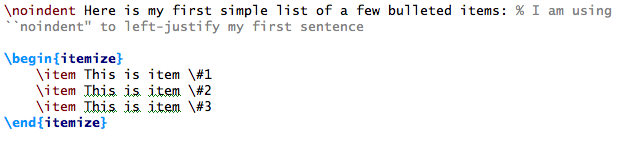
\includegraphics[scale=.6]{CODE8} \\
	\centering
\end{figure}

This gives us the output, \\

\begin{figure}[!h]
	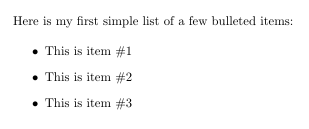
\includegraphics[scale=.6]{OUT8} \\
	\centering
\end{figure}

As we would expect, we have a bulleted list with each of our items. Notice my comment after the main setnece (followed by the ``\%" sign). \LaTeX\ automatically indents, so if you don't want this, simply type the command ``noindent" following the backslash as we would with any other command. Also, note that we have to essentially treat the pound sign (``\#") as a command, to avoid errors. This is the same as using the dollar sign (``\$"), the ampersand (``\&"), and so on. Otherwise, it will treat those as delimiters as we have seen throughout. \\

\subsection{Centering Lists}

\forceindent Now let's say we wanted to center our list under some text. As with drawing tables, we would simply include the command ``centering." To see this, let's update our simple code with the following,

\begin{figure}[!h]
	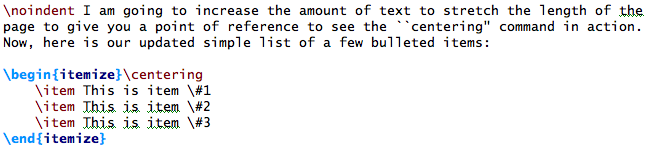
\includegraphics[scale=.6]{CODE9} \\
	\centering
\end{figure}

This gives us the output, \\

\begin{figure}[!h]
	
\includegraphics[scale=.6]{OUT9} \\
	\centering
\end{figure}

\subsection{Nesting Lists}

A final note on itemized lists (or also for numbered lists addressed below). As they are generated using environments, remember back to the beginning when we noted that environments can be nested. Thus, if we wanted to nest a list within a list, we would simply start a new environment within our base ``itemize" environment. Let's update our code,

\begin{figure}[!h]
	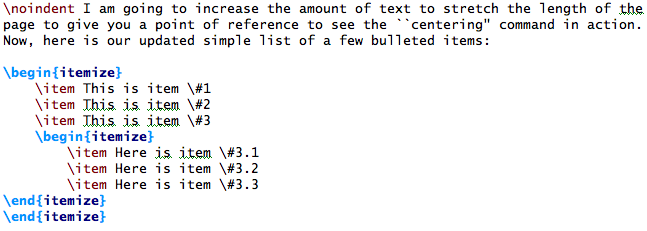
\includegraphics[scale=.6]{CODE10} \\
	\centering
\end{figure}

This gives us the output, \\

\begin{figure}[!h]
	
\includegraphics[scale=.6]{OUT10} \\
	\centering
\end{figure}

\newpage 

\section{Numbering}

\subsection{Basics of ``Enumerate"}

\forceindent Finally, what if we want to number our list? Well, all we need to do is change the environment from ``itemize" to ``enumerate." All other syntax remains the same. So, let's see this by updating our nested original table previously used for our itemized list. Type,

\begin{figure}[!h]
	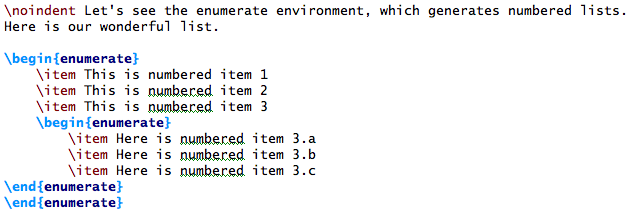
\includegraphics[scale=.6]{CODE11} \\
	\centering
\end{figure}

Now we see our same list, only numbered, \\

\begin{figure}[!h]
	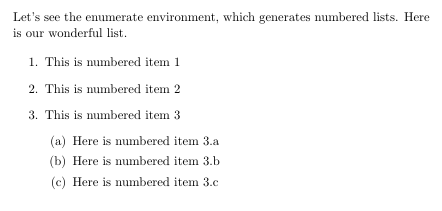
\includegraphics[scale=.6]{OUT11} \\
	\centering
\end{figure}

\subsection{A Few Extras on ``Enumerate"}

\forceindent If you wanted to ``list" certain items, but didn't want any counter or bullets (from ``itemize"), you simply type an open and closed bracket after each item in your environment. Also, if you wanted to change the sub-list from letters (default) to numbers, you need to first load the enumerate package (as opposed to just accessing the environment as we have been doing), and then type in the brackets placed outside the enumerate environment beginning, the number or letter you want to start. \\

So first, before we see everything together, type the following to load our ``short labels" options,

\begin{figure}[!h]
	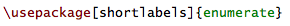
\includegraphics[scale=.6]{CODE12} \\
	\centering
\end{figure}

Now, with that loaded, we can do both of the additions/changes to our list as addressed above, with the following code. Type,

\begin{figure}[!h]
	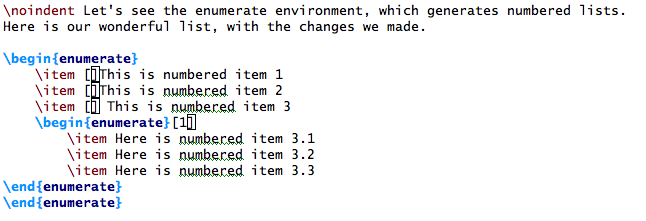
\includegraphics[scale=.6]{CODE13} \\
	\centering
\end{figure}

Now we see our updated numbered list,\footnote{Note that you may get a warning message saying it couldn't find or use ``shortlabels." But check to see that your output is as you think it should be. If it looks fine, then just disregard this warning from \TeX\ Studio.} \\

\begin{figure}[!h]
	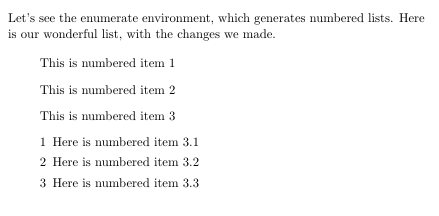
\includegraphics[scale=.6]{OUT13} \\
	\centering
\end{figure}

\end{document}
